

\section{Outline}

\begin{frame}
  \centering
  {\huge
    Programming Challenges Tips and Tricks
  }
\end{frame}

\begin{frame}[t]{Week 1: Tips for Programming Challenges}

  First week: 7 Easy problems (1 long problem)! What do you need to learn?
  \bigskip

  \begin{enumerate}
    \item How to read a program challenge? (Problem style)
    \item How to use the Automated Judge? (Input and Output)
    \item How to debug? (Thinking and Debug Data)
  \end{enumerate}
  \bigskip

  The class one material contains \alert{General Tips} for this course.
  \medskip

  These Tips will be useful for the rest of the course. Learn them well!
\end{frame}

\begin{frame}{Topics for today}
  \begin{itemize}
    \item Tip 1: Reading the problem;
    \item Tip 2: Problem size and algorithm analysis;
    \item Tip 3: Writing test cases;
    \item Tip 4: Input/Output;
    \item Tip 5: How to ask for help;
  \end{itemize}
\end{frame}

\section{Tip 1: Reading the Problem}
\begin{frame}{Tip 1: Reading, Thinking, then Coding}

  \begin{columns}
    \column{0.7\textwidth}
    \begin{itemize}
    \item It is very important to \alert{read and understand the problem} before start coding.

    \item If you completely understand the problem, you can avoid small mistakes.
    
    \item Maybe read the \alert{Input and Output} first!

    \item Try to solve the problem \alert{on paper}

    \item If you don't understand the problem, ask for help!
    
    \item Quickly read all 8 problems before starting. Different people like different problems.
    \end{itemize}
    \column{0.3\textwidth}
    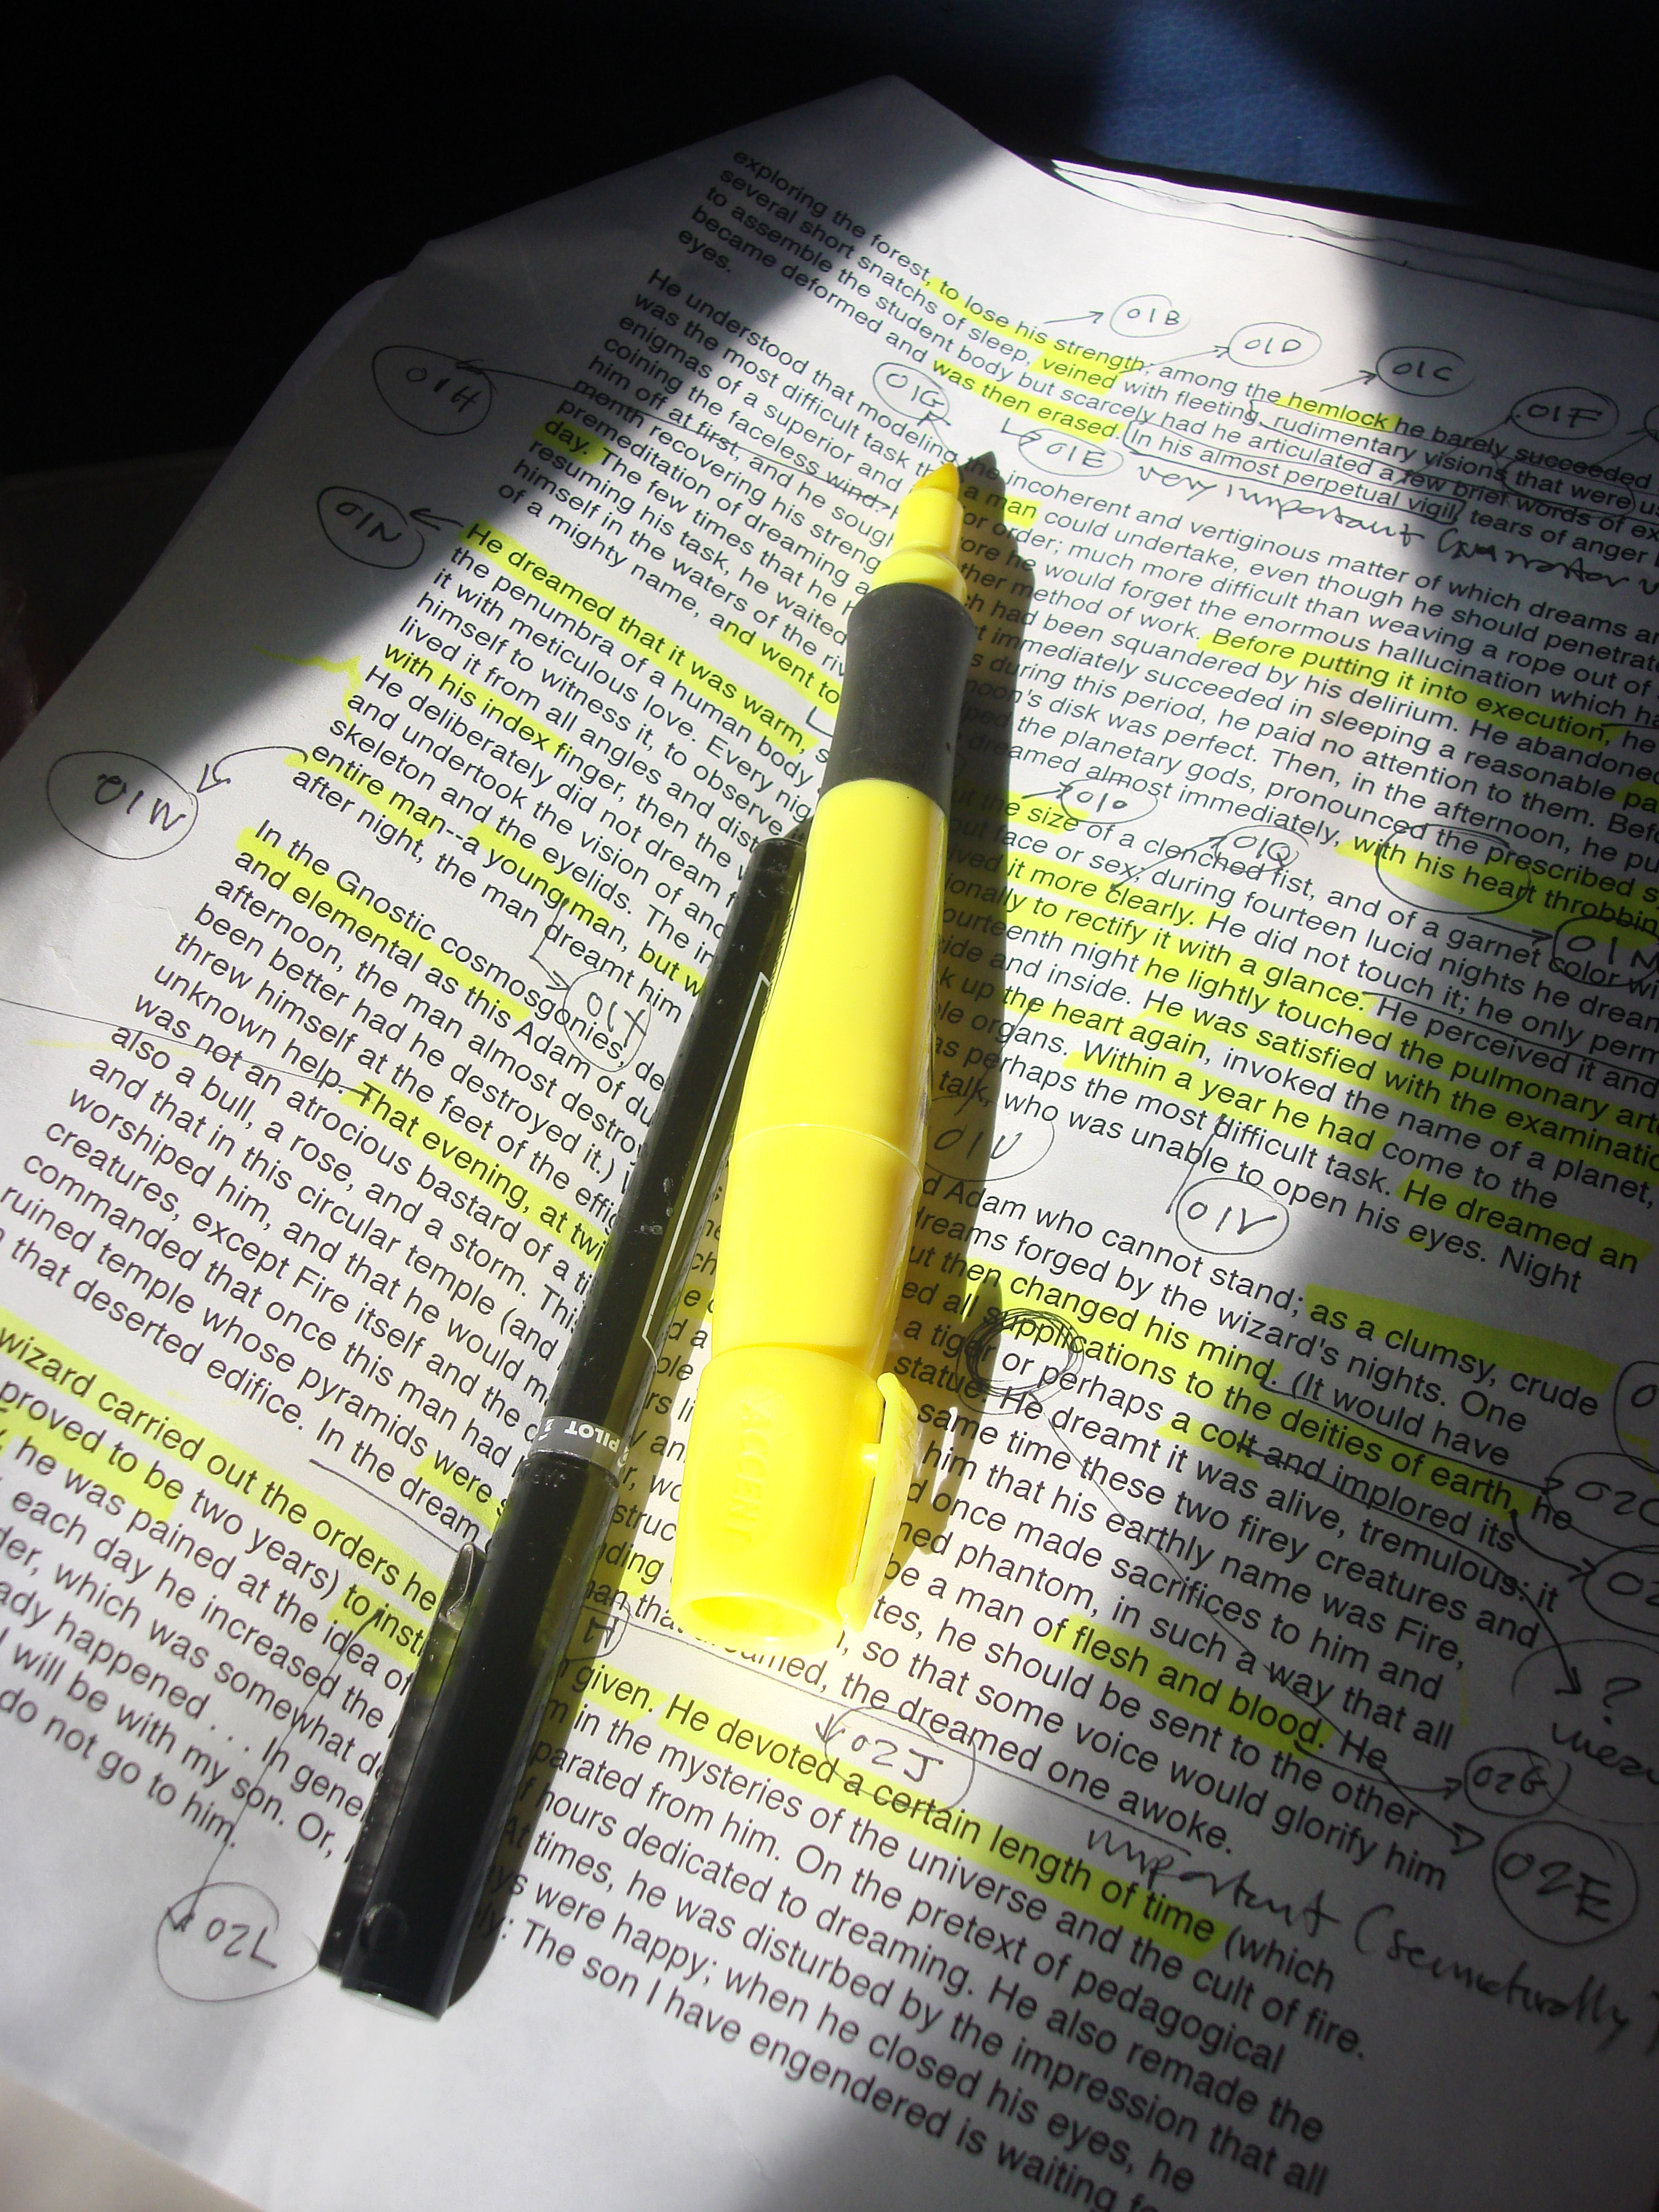
\includegraphics[width=\textwidth]{../img/textmarker}
  \end{columns}

  \vfill

  \hrulefill\\
  \hfill {\tiny Image by Guido ``random'' Alvarez, released as CC-BY-2.0}
\end{frame}

% \begin{frame}
%   \frametitle{Tricks for reading the problem}

%   \begin{alertblock}{}
%     Reading problems in English is hard :-(
%   \end{alertblock}

%   \begin{itemize}
%     \item Don't worry: deepl and google translate can help!
%     \begin{itemize}
%       \item Be careful, sometimes they are wrong...
%     \end{itemize}\medskip

%     \item Separate {\bf story} from {\bf problem}
%     \begin{itemize}
%       \item Look for keywords: Maximum, Total, Cost, Rules, Number, Constraint, etc...
%     \end{itemize}\medskip

%     \item Read the {\bf Input} and {\bf Output} section first!
%     \begin{itemize}
%       \item Sometimes you can understand the problem just from input/output.
%       \item But be careful of special rules!
%     \end{itemize}\medskip

%     \item Understanding a little English is good for Computer Science;

%   \end{itemize}
% \end{frame}

\section{Tip 2: Think about the problem size!}

\begin{frame}{Hint 2: Be careful of problem size!}
  Some of the secret input sizes are very big. \bigskip

  If your program is too slow, you cannot solve big input sizes.\bigskip 

  When you read the problem, \alert{pay attention to the input size}.\bigskip

  Think about the \alert{the number of loops} that your program uses!
\end{frame}


%\item Hint 2: Problem size and algorithm analysis;

\subsection{Revisiting the 3n+1 problem}

\begin{frame}[fragile]{Program is too slow: Example 1}

  \begin{block}{}
    Calculate the {\bf Maximum Execution Length} between any two numbers $i$ and $j$.
  \end{block}
  \smallskip

\begin{verbatim}
Execution of (n)
1. print n
2. if n == 1 then STOP
3. if n is odd then n = 3n + 1
4. else n = n/2
5. GOTO 2

Example: Execution of (22)
22 11 34 17 52 26 13 40 20 10 5 16 8 4 2 1 -- Execution Length = 16
\end{verbatim}
For {\bf ONE} input, the problem is small and easy.
\end{frame}

\begin{frame}[fragile]
  \frametitle{A simple solution for the 3n+1 problem}
  \begin{columns}
    \column{0.4\textwidth}
    Simple solution: loop until n == 1 and count the loops (lines 9-12).\bigskip

    However, for large input, this program is too slow.\bigskip

    \alert{Remember}: You have to execute the program for \alert{every input} between $i$ and $j$
    \column{0.6\textwidth}
  {\smaller
\begin{verbatim}
 1 while true:
 2  try:
 3    line = input()
 4    max = 0
 5    tk = line.split()
 6    i, j = int(tk[0]), int(tk[1])
 7    for n in range(i, j+1):
 8      count = 1
 9      while n != 1:
10        if n % 2 == 1: n = 3 * n + 1
11        else: n = n / 2
12        count += 1
13      if count > max: max = count
14    print (line, max)
15  except EOFError: break
\end{verbatim}}
\end{columns}
\end{frame}

%%%%%%%%%%%
\begin{frame}[fragile]
  \frametitle{Large input in the 3n+1 problem}

    \begin{itemize}
      \item Objective: Calculate the largest execution between $i$ and $j$. For a large input:
    \begin{verbatim}
Input: 1 10000 <-- Largest between 1 and 10000?
Output: 262    <-- Largest is 262 steps
    \end{verbatim}

      \item 262 steps for 1 execution is short.\\
      But for 10000 inputs: $262\times10000 = 2,000,000$ steps!\medskip

      \item Can we make it faster?


    \end{itemize}
\end{frame}

\begin{frame}[fragile]
  \frametitle{Make 3n+1 faster by removing repetition}

  \begin{itemize}
    \item Some examples of calculating (A(n)) -- Note the repetition:
\begin{verbatim}
A(22):  22 11 34 17 52 26 13 40 20 10 5 16 8 4 2 1
A(11):  11 34 17 52 26 13 40 20 10 5 16 8 4 2 1
A(17):  17 52 26 13 40 20 10 5 16 8 4 2 1
A(13):  13 40 20 10 5 16 8 4 2 1
A(10):  10 5 16 8 4 2 1
A(8) :  8 4 2 1
\end{verbatim}\medskip

    \item To avoid the repetition, \alert{we store partial results in an array}.
    \medskip

    \item This technique is called {\bf Memoization}. It is very useful for many problems!
  \end{itemize}

\end{frame}

\begin{frame}[fragile]{Memoization for 3n+1}
  Use a list or dictionary to memorize past results ({\bf memo table}). Check the memo table before calculating results.
\begin{verbatim}
  memotable = {}
  memotable[1] = 1

  def A(n):
    if n in table.keys(): return table[n]
    else:
      if n % 2 == 1: table[n] = 1 + A(3*n + 1)
      else: table[n] = 1 + A(n/2)
    return table[n]
\end{verbatim}
More about Memo Tables in Lecture 4 (Dynamic Programming)
\end{frame}


\subsection{Problem Size Example 2: 8-Queens}

\begin{frame}[fragile]{Problem Size Example: 8 Queen Problem}
  \begin{columns}
    \column{0.8\textwidth}
    8-Queen problem: Place 8 queens in a chess board, so that {\bf all columns, all rows, and all diagonals are different}\bigskip

    {\bf Algorithm (1)}: Eight loops size 64: Try all rows and all columns for queen 1, queen 2, queen 3, queen 4, ... etc.
    \column{0.2\textwidth}
    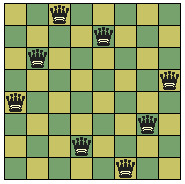
\includegraphics[width=1\textwidth]{img/8queen}
  \end{columns}
\begin{verbatim}
Choices for Queen1: a1, a2, a3, a4, ..., h6, h7, h8
Choices for Queen2: a1, a2, a3, a4, ..., h6, h7, h8
Choices for Queen3: a1, a2, a3, a4, ..., h6, h7, h8
...
Choices for Queen8: a1, a2, a3, a4, ..., h6, h7, h8

Total Number of choices: 64 x 64 x 64 x 64 = 64^8 ~ 10^14
                                        TOO MANY!
\end{verbatim}
\end{frame}

\begin{frame}[fragile]{Reducing the size of 8-Queen (1)}

  \begin{columns}
    \column{0.8\textwidth}
    To reduce the number of choices, we force each queen to be on a different row, and only choose the column.\bigskip

    {\bf Algorithm (2)}: Eight loops size 8: Try all columns for queen 1 (fix row 1), all columns for queen 2 (fix row 2), ..., etc.
    \column{0.2\textwidth}
    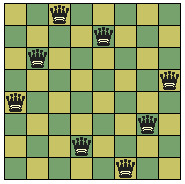
\includegraphics[width=1\textwidth]{img/8queen}
  \end{columns}
\begin{verbatim}
Choices for Queen1: a1, b1, c1, d1, e1, f1, g1 or h1
Choices for Queen1: a2, b2, c2, d2, e2, f2, g2 or h2
Choices for Queen1: a3, b3, c3, d3, e3, f3, g3 or h3
...
Choices for Queen8: a8, b8, c8, d8, e8, f8, g8 or h8

Total Solutions: 8 x 8 x 8 ... = 8^8 ~ 10^7
                                    Still Big!
\end{verbatim}
\end{frame}

\begin{frame}[fragile]{Reducing the size of 8-Queen (2)}
  \begin{columns}
    \column{0.8\textwidth}
      We can reduce the number of choices even more, if we force the columnd and the row of each queen to be different.\bigskip

    {\bf Algorithm (3)}: Fix the row for each queen, 1 loop through the \alert{permutation} of columns.
    \column{0.2\textwidth}
    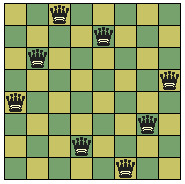
\includegraphics[width=1\textwidth]{img/8queen}
  \end{columns}
\begin{verbatim}
Choice 1: {a1, b2, c3, d4, e5, f6, g7, h8}
Choice 2: {a1, b2, c3, d4, e5, f6, g8, h7}
Choice 3: {a1, b2, c3, d4, e5, f7, g6, h8}
Choice 4: {a1, b2, c3, d4, e5, f7, g8, h6}
...

Total Solutions: 8 x 7 x 6 x 5 ... = 40320  --  OK!
\end{verbatim}
\end{frame}

\begin{frame}{Reducing the size of 8-Queen: Summary}

  \hfill 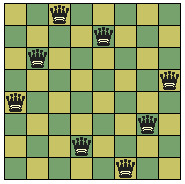
\includegraphics[width=0.2\textwidth]{img/8queen}
  \begin{itemize}
    \item Algorithm 1: All rows and columns: $10^{14}$ steps;
    \item Algorithm 2: Fix rows, All columns: $10^{7}$ steps;
    \item Algorithm 3: Permutation: 40320 steps;
  \end{itemize}
\end{frame}

% \begin{frame}{How many steps is too slow?}{$lt$ 10.000.000 steps is a good goal}

%   \begin{block}{n $<$ 24}
%     Almost anything works: Brute force! (Maybe not factorial)
%   \end{block}

%   \begin{block}{n = 500}
%     Cubic algorithms are too big (O($n^3$) = 125.000.000).
%     Maybe O($n^2\text{log}n$).
%   \end{block}

%   \begin{block}{n = 10.000}
%     A square algorithm (O($n^2$)) is still okay. Be careful of big constants!
%   \end{block}

%   \begin{block}{n = 1.000.000}
%     O($n$log$n$) = 13.000.000. We might need a linear algorithm!
%   \end{block}
% \end{frame}

%%%%%%%%%%%%%%%%%%%%%%%%%%%
%\item Hint 3: Writing test cases;
\section{Hint 3: Writing test cases}

\begin{frame}{Hint 3: Write testcases!}

  The description of a problem includes \alert{Sample Input}.\bigskip

  However, the judge checks your program with \alert{Test Input}.\bigskip

  \begin{exampleblock}{Example: 3n+1 Problem}
    Sample Input: always $i < j$.\medskip

    Hidden Input: sometimes $i > j$!\medskip
  \end{exampleblock}\bigskip

  \alert{The Test Input is more difficult than the Sample Input}!

\end{frame}

% Extend basic Cases
% Write extreme cases (maxcase, etc)
% write cases where you think a bug might be
% write random cases

\begin{frame}{The Test Input is more difficult than the Sample Input!}

    \begin{itemize}
      \item Input is Negative; Input is Minimum; Input is Maximum;
      \item Input is out of order, Input is in reverse order;
      \item Input is repeated;\medskip

      \item Graph is disconnected; Graph is fully connected;
      \item Lines are parallel; Points are in the same place;
      \item Angle is 0; Area is 0;\medskip
    \end{itemize}

    \begin{block}{}
      Read the input rule carefully.\medskip
      
      Create your own \alert{Debug Input}
    \end{block}
\end{frame}

\begin{frame}
  \frametitle{Creating Debug Input}

  Create and test a \alert{Debug Input} before submitting the program!\bigskip

  Many wrong programs can be fixed if you create debug input before submitting.\bigskip

  Again: \alert{Create Debug Input!}

  \begin{exampleblock}{Ideas for Debug Input (checklist)}
    \begin{itemize}
      \item Simple Debug Input;
      \item Debug Input with maximum value;
      \item Debug Input with tricky cases;
      \item Random Debug Input Input (use scripts!);
    \end{itemize}
  \end{exampleblock}

  Creating debug input is an important skill for research and work!
\end{frame}

%%%%%%%%%%%%%%%%%%%%%%%%%%%%%%%%%%%%%%%%%%%%%

%\item Hint 4: Input/Output;

% # Dealing with IO
% ## Standard IO Types (https://github.com/stevenhalim/cpbook-code/tree/master/ch1/ch1IO.cpp)
%
% ## Basic String Skills(https://github.com/stevenhalim/cpbook-code/tree/master/ch1/basic_string.cpp)
%
% ## Be careful of output:
% - Case
% - Number of decimal places: Round up or down
% - Tie breakers

\section{Hint 4: Input and Output}
\begin{frame}
  \frametitle{Tip 4: Read the Input and Output description carefully}

  \begin{itemize}
  \item What is the stop condition?
  \begin{itemize}
    \item The number of inputs is given in the beginning;
    \item Special value to indicate the end of the input;
    \item Input ends at the end of the file (EOF);
  \end{itemize}
  \medskip

  \item What is the format of the input/output?
  \begin{itemize}
    \item Very important for output (floating point precision)
  \end{itemize}
  \medskip

  \item What is the size of the input?
  \begin{itemize}
    \item What is the maximum number of inputs?
    \item What are the maximum and minimum values?
    \item Are there special conditions?
  \end{itemize}
  \end{itemize}
\end{frame}


\begin{frame}[fragile]
  \frametitle{There are 3 common stop conditions}

  \begin{enumerate}
  \item Read $N$, then read $N$ queries;
\begin{verbatim}
int n; cin >> n;
for (; n > 0; n--) { // Do something }
\end{verbatim}
\item Read until a special condition; (example, until $n = 0$)
\begin{verbatim}
int n; cin >> n;
while (n != 0) { // Do something
cin >> n; }
\end{verbatim}
  \item Continue reading until no more Input\hfil (Until EOF);
\begin{verbatim}
int a, b;
while (cin >> a >> b;) { // Do something! }
\end{verbatim}
  \end{enumerate}
\end{frame}

\begin{frame}
  \frametitle{Output: You need to return EXACTLY what the problem requires}
  \begin{columns}
    \column{0.2\textwidth}
  
\includegraphics[width=1\textwidth]{../img/angryclient}
    \column{0.8\textwidth}

  Be careful with the common mistakes:\medskip
  \begin{itemize}
    \item REMOVE PRINT DEBUG.\medskip

    \item UPPERCASE vs lowercase
    \item Singular vs plural
    \item Start with 1 vs start with 0
    \medskip

    \item Number of float digits: 0.34 x 0.340
    \item Round up or round down?: 0.34 x 0.35
    \medskip

    \item Solution order;\medskip

    \item etc...
  \end{itemize}
  \end{columns}
\end{frame}

%%%%%%%%%%%%%%%%%%%%%%%%%%%%%%%%%%%%%%%%%%%%

\section{Hint 5: How to ask for help}

\begin{frame}{Tip 5: How to ask for help}

  When you are stuck, it is okay to ask for help from the teacher or from your friends.\bigskip

  When you ask for help, add as much information as you can about your problem.\bigskip

  (This is a training for bug reporting as well!)\bigskip

  \begin{block}{Help Checklist}
  \begin{enumerate}
    \item Send your current code. (Do not send screenshot!)\medskip

    \item Explain the idea of your program.\medskip

    \item Explain the Debug Input you used.\medskip
  \end{enumerate}
  \end{block}
\end{frame}

\section{Conclusion}

\begin{frame}\frametitle{Final message}
  Thank you for listening!\vfill

  Have fun writing programs.\vfill

  Be faster than your friends!\vfill

  Ask questions on manaba.
\end{frame}
